\documentclass[11pt,a4paper]{article}
\usepackage[T1]{fontenc}
\usepackage{lmodern}
\usepackage[margin=2.3cm]{geometry}
\usepackage{microtype}
\usepackage{amsmath}
\usepackage{graphicx}
\usepackage{xcolor}
\usepackage{enumitem}
\usepackage[colorlinks=true,urlcolor=blue!50!black,linkcolor=black]{hyperref}
\graphicspath{{../figures/}}
\setlength{\parindent}{0pt}
\setlength{\parskip}{0.7em}
\pagestyle{plain}

\begin{document}

\begin{center}
{\LARGE\bfseries Fossils in a Spinning Galaxy:\\[0.3em] Finding the Milky Way's Oldest Building Blocks with Gaia DR4}
\end{center}
\vspace{0.5em}

The Milky Way grew by swallowing smaller galaxies and star clusters. As each one fell in, the Galaxy's tides pulled it apart, and its stars spread out into the diffuse stellar halo that surrounds the disc. Seen on the sky, the debris from different victims is now thoroughly mixed. Yet each star still carries a memory of where it came from, and Galactic archaeology sets out to read that memory and reconstruct how our Galaxy was assembled (Freeman \& Bland-Hawthorn 2002; Helmi 2020). The aim of this project is to discover the oldest of these remnants, hidden in the inner Galaxy, in the new Gaia data release due during the academic year. The same data can then show what each remnant was, and how the Galaxy's central bar has rotated and slowed.

The memory is stored in the conserved quantities of each star's orbit. If the Galaxy's gravitational potential $\Phi$ does not change with time, a star's energy per unit mass,
\begin{equation}
E = \tfrac{1}{2}|\mathbf{v}|^2 + \Phi(\mathbf{x}),
\end{equation}
stays constant; if the potential is also symmetric about the rotation axis, so does the $z$-component of angular momentum, $L_z = x v_y - y v_x$. Stars torn from the same dwarf galaxy started with similar $E$ and $L_z$, and they keep them long after they have spread around the sky. Plot the halo stars in the $E$--$L_z$ plane and the shredded galaxies reappear as distinct clumps (Helmi et al.\ 1999; Helmi \& de Zeeuw 2000). The Gaia satellite, which measures the positions and velocities of stars in three dimensions, turned this idea into a discovery machine. It revealed that a large dwarf galaxy, Gaia--Sausage--Enceladus, merged with the Milky Way roughly ten billion years ago and supplied most of the inner halo (Belokurov et al.\ 2018; Helmi et al.\ 2018), and a series of smaller accreted structures soon followed (e.g.\ Myeong et al.\ 2019).

This method fails in the inner Galaxy, where much of the debris should lie. The inner Milky Way contains a bar, an elongated structure of stars that rotates as a solid body with a pattern speed $\Omega_\mathrm{b}$. A rotating bar makes the potential depend on time, so neither $E$ nor $L_z$ is conserved. Dillamore \& Sanders (2025) worked out how much this matters. They studied an analytic model, simulations of stars orbiting in steady and slowing bars, and a cosmological simulation of a Milky Way-like galaxy. All three give the same answer: the bar increases the spread in $E$ and $L_z$ of a single progenitor's debris by a factor of ten to a hundred, so a clump that should stand out blends into the smooth halo. The worst-affected orbits are those more tightly bound than the Sun's, with energies below the Sun's orbital energy and apocentres within about 40\,kpc. Orbits that are prograde, eccentric, or close to the disc plane suffer most. About three quarters of the Milky Way's globular clusters, and a quarter of its known stellar streams, move on such orbits.

The bar has not destroyed this debris. It has scrambled the debris in the very coordinates used to search for it. The substructure found so far comes mainly from the outer, higher-energy halo, where $E$ and $L_z$ still work. Inside the Solar radius, the remains of the earliest accreted dwarf galaxies and of dissolved star clusters, which record the Galaxy's first billion years, have been erased from the $E$--$L_z$ maps. Dillamore \& Sanders predict that such bar-dispersed substructure is abundant. Most of the substructure in the inner Milky Way is therefore probably still undiscovered, and this is the main opportunity of the project. A new search must also avoid false detections: the bar drives some halo stars into chaotic orbits (Woudenberg \& Helmi 2025) and, through its resonances, can create clumps that come from no progenitor at all (Dillamore et al.\ 2023, 2025).

Classical mechanics offers a cure. In a frame rotating with the bar, the potential is static, so the energy in that frame is conserved. Expressed in the inertial-frame quantities above, this conserved quantity is the Jacobi integral,
\begin{equation}
H_\mathrm{J} = E - \Omega_\mathrm{b} L_z ,
\end{equation}
familiar from the restricted three-body problem. Dillamore \& Sanders (2025) tested $H_\mathrm{J}$ in an analytic model, in simulations of stars orbiting in a steady and a slowing bar, and in a cosmological simulation of a Milky Way-like galaxy. In each case, debris that the bar smears out in $E$--$L_z$ stays compact in $H_\mathrm{J}$: exactly when the bar turns steadily, and to a good approximation when it slows down.

\begin{figure}[t]
\centering
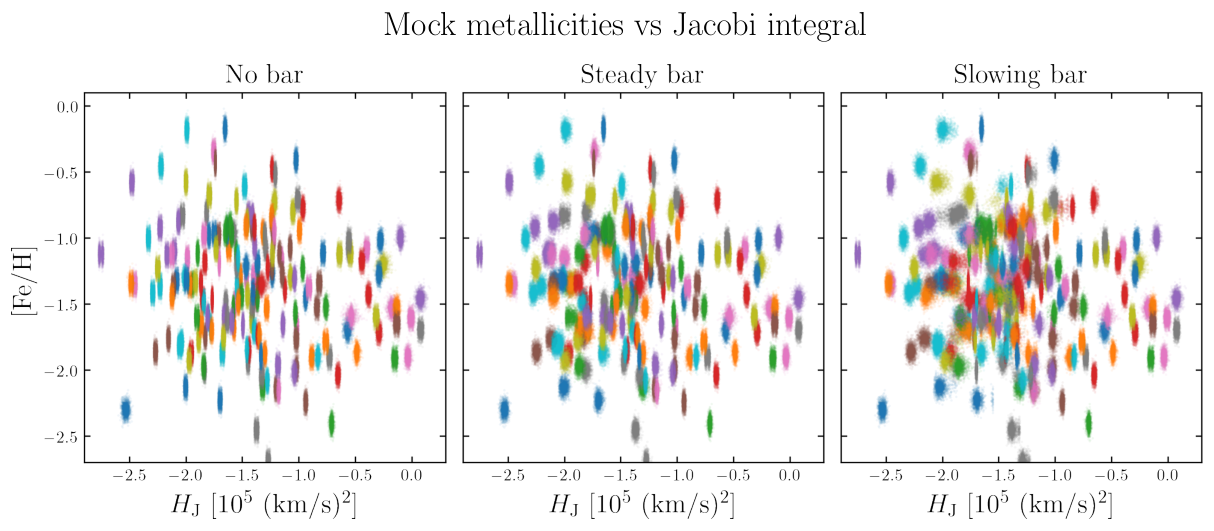
\includegraphics[width=\textwidth]{05_dillamore_sanders_HJ_FeH.png}
\caption{\small Simulated debris from 200 disrupted star clusters in the plane of metallicity [Fe/H] and Jacobi integral $H_\mathrm{J}$, for no bar, a steady bar, and a slowing bar. Each colour is one progenitor. The debris stays in tight clumps even when the bar slows, although the same stars are smeared out in $E$--$L_z$. This is the signal the project searches for in Gaia DR4. From Dillamore \& Sanders (2025).}
\label{fig:hj}
\end{figure}

Chemistry adds a second, independent record that the bar cannot alter. A star's surface composition is set by the gas it formed from. Astronomers write the iron abundance relative to the Sun as $[\mathrm{Fe/H}] = \log_{10}(N_\mathrm{Fe}/N_\mathrm{H})_\star - \log_{10}(N_\mathrm{Fe}/N_\mathrm{H})_\odot$, so a star with $[\mathrm{Fe/H}] = -2$ has one hundredth of the Sun's iron. Each progenitor formed its stars over a different history, and so left a different chemical signature: dwarf galaxies show a characteristic drop in the ratio of $\alpha$-elements (such as magnesium) to iron, while dissolved globular clusters leave stars rich in nitrogen and aluminium (Belokurov \& Kravtsov 2023). A group of stars that clumps both in $H_\mathrm{J}$ and in chemistry, as in Figure~\ref{fig:hj}, is a strong candidate for a genuine fossil.

So far, too few stars have full three-dimensional velocities to apply this idea to the inner Galaxy. Gaia's fourth data release, DR4, due on 2 December 2026, will change that. It is based on 5.5 years of observations and will contain far more precise distances, motions, and radial velocities than any earlier catalogue. The student will combine these with chemical abundances from the large spectroscopic surveys (Gaia's own spectra, APOGEE, GALAH, LAMOST, and DESI). During the first term they will build a pilot sample from Gaia DR3 and APOGEE and test the method on simulated data; from January they will apply it to DR4. No one has yet searched the inner halo in $H_\mathrm{J}$ and chemistry with a sample of this size, so any structure that survives the tests will be a new discovery.

The project uses an existing, tested Python framework built on the galaxy-modelling package AGAMA (Vasiliev 2019). The student will compute $E$, $L_z$, and $H_\mathrm{J}$ for each star in a realistic model of the Galaxy's potential, over a range of possible bar pattern speeds. To decide whether the clumps are real, they will compare the data with shuffled copies in which the link between $H_\mathrm{J}$ and metallicity is broken at random; real debris should make the data more clustered than any shuffled copy. Simulated debris injected into the catalogue will show how well the method recovers real structure and how often noise creates false clumps. The strongest candidates will then be examined star by star in their orbits and detailed chemistry. The goal is the first list of ancient relics hidden in the inner halo. If none survive, the project will set firm limits on how many can exist; either answer constrains how many systems built the young Milky Way and how massive they were.

Once the search is complete, the student can extend the project in one of two directions.

The first extension asks \emph{what the clumps are}. Chemistry can tell the two main kinds of progenitor apart. A dissolved globular cluster leaves stars with almost the same metallicity, enhanced in nitrogen and aluminium and depleted in carbon. A dwarf galaxy formed stars over a longer time, so its debris spans a range of metallicity and shows a drop in [$\alpha$/Fe] at higher [Fe/H]. Among dwarf galaxies, more massive systems reach higher metallicity (Kirby et al.\ 2013), so the chemistry of a clump also estimates the mass of its progenitor, from an ultra-faint dwarf to a galaxy as massive as Gaia--Sausage--Enceladus. The inner Galaxy already shows hints of both kinds of debris. It contains many nitrogen-rich field stars, which may come from dissolved globular clusters whose total mass exceeds that of the surviving clusters several times over (Schiavon et al.\ 2017; Belokurov \& Kravtsov 2023), and chemistry has revealed the remains of a massive early accreted galaxy buried within about 4\,kpc of the Galactic centre (Horta et al.\ 2021). Classifying the new clumps one by one, and comparing their orbits with those of surviving globular clusters and dwarf galaxies, would turn the discovery list into a census of the Galaxy's earliest building blocks: how many were star clusters, how many were dwarf galaxies, and how massive they were.

The second extension measures \emph{the bar and its coupling to the dark-matter halo}. $H_\mathrm{J}$ is conserved only when it is computed with the bar's true pattern speed. With the wrong $\Omega_\mathrm{b}$, each clump of debris spreads out again, so the clustering signal is strongest at the true value. The pattern speed is still uncertain. Early estimates from the motions of nearby stars favoured a fast bar, above $50\,\mathrm{km\,s^{-1}\,kpc^{-1}}$ (Dehnen 2000); recent measurements from stars in the bar region give about $39$--$41\,\mathrm{km\,s^{-1}\,kpc^{-1}}$ (Portail et al.\ 2017; Sanders, Smith \& Evans 2019; Bovy et al.\ 2019), with systematic errors of 5--10 $\mathrm{km\,s^{-1}\,kpc^{-1}}$.

The bar is also expected to slow down, and its slowing links it to the dark matter. It exchanges angular momentum with stars and dark matter on resonant orbits, and dynamical friction from the dark-matter halo drains its angular momentum and brakes its rotation (Weinberg 1985; Debattista \& Sellwood 2000). How fast it slows depends on how much dark matter lies near the bar's resonances and how fast that dark matter moves (Athanassoula 2003), and the braking torque can oscillate over billions of years as dark matter trapped in the resonances sloshes back and forth (Chiba \& Schönrich 2022). From the motions of disc stars, Chiba, Friske \& Schönrich (2021) estimated that the Milky Way's bar is slowing by $4.5 \pm 1.4\,\mathrm{km\,s^{-1}\,kpc^{-1}}$ per billion years. Halo debris offers an independent record. Halo stars, like dark-matter particles, are collisionless and feel the bar's torque in the same way, and in the $E$--$L_z$ plane the bar spreads each clump along a line of slope $\mathrm{d}E/\mathrm{d}L_z = \Omega_\mathrm{b}$. Comparing the observed debris with simulations of steady and slowing bars (Dillamore \& Sanders 2025) can therefore constrain both the present pattern speed and its past evolution, and through them the density of dark matter in the inner Galaxy. The student will claim a value only if it survives changes in the measurement errors, the assumed Galactic potential, and the sample, since the injection tests show that large errors can create a false peak.

The project suits a student who enjoyed Part II classical mechanics and likes programming in Python. Previous study of Galactic dynamics is useful but not required.

\vspace{0.5em}
{\small\raggedright
\textbf{Further reading}
\begin{itemize}[leftmargin=1.2em,itemsep=0.1em,parsep=0pt,topsep=0.3em]
\item Helmi, A. (2020), \emph{Streams, Substructures, and the Early History of the Milky Way}, ARA\&A, 58, 205. \href{https://doi.org/10.1146/annurev-astro-032620-021917}{doi:10.1146/annurev-astro-032620-021917}
\item Freeman, K. \& Bland-Hawthorn, J. (2002), \emph{The New Galaxy: Signatures of Its Formation}, ARA\&A, 40, 487. \href{https://doi.org/10.1146/annurev.astro.40.060401.093840}{doi:10.1146/annurev.astro.40.060401.093840}
\item Dillamore, A.\,M. \& Sanders, J.\,L. (2025), \emph{Bar-driven dispersal of Galactic substructure}, MNRAS, 542, 1331. \href{https://doi.org/10.1093/mnras/staf1264}{doi:10.1093/mnras/staf1264}
\item Woudenberg, H.\,C. \& Helmi, A. (2025), \emph{The chaotic motion of nearby halo stars due to the Galactic bar}, A\&A, 700, A240. \href{https://doi.org/10.1051/0004-6361/202555672}{doi:10.1051/0004-6361/202555672}
\item Dillamore, A.\,M. et al.\ (2023), \emph{Stellar halo substructure generated by bar resonances}, MNRAS, 524, 3596. \href{https://doi.org/10.1093/mnras/stad2136}{doi:10.1093/mnras/stad2136}
\item Dillamore, A.\,M. et al.\ (2025), \emph{Dynamical streams in the local stellar halo}, MNRAS, 541, 214. \href{https://doi.org/10.1093/mnras/staf965}{doi:10.1093/mnras/staf965}
\item Helmi, A., White, S.\,D.\,M., de Zeeuw, P.\,T. \& Zhao, H. (1999), \emph{Debris streams in the solar neighbourhood as relicts from the formation of the Milky Way}, Nature, 402, 53. \href{https://doi.org/10.1038/46980}{doi:10.1038/46980}
\item Helmi, A. \& de Zeeuw, P.\,T. (2000), \emph{Mapping the substructure in the Galactic halo with the next generation of astrometric satellites}, MNRAS, 319, 657. \href{https://doi.org/10.1046/j.1365-8711.2000.03895.x}{doi:10.1046/j.1365-8711.2000.03895.x}
\item Belokurov, V., Erkal, D., Evans, N.\,W., Koposov, S.\,E. \& Deason, A.\,J. (2018), \emph{Co-formation of the disc and the stellar halo}, MNRAS, 478, 611. \href{https://doi.org/10.1093/mnras/sty982}{doi:10.1093/mnras/sty982}
\item Helmi, A. et al.\ (2018), \emph{The merger that led to the formation of the Milky Way's inner stellar halo and thick disk}, Nature, 563, 85. \href{https://doi.org/10.1038/s41586-018-0625-x}{doi:10.1038/s41586-018-0625-x}
\item Myeong, G.\,C., Vasiliev, E., Iorio, G., Evans, N.\,W. \& Belokurov, V. (2019), \emph{Evidence for two early accretion events that built the Milky Way stellar halo}, MNRAS, 488, 1235. \href{https://doi.org/10.1093/mnras/stz1770}{doi:10.1093/mnras/stz1770}
\item Belokurov, V. \& Kravtsov, A. (2023), \emph{Nitrogen enrichment and clustered star formation at the dawn of the Galaxy}, MNRAS, 525, 4456. \href{https://doi.org/10.1093/mnras/stad2241}{doi:10.1093/mnras/stad2241}
\item Dehnen, W. (2000), \emph{The Effect of the Outer Lindblad Resonance of the Galactic Bar on the Local Stellar Velocity Distribution}, AJ, 119, 800. \href{https://doi.org/10.1086/301226}{doi:10.1086/301226}
\item Portail, M., Gerhard, O., Wegg, C. \& Ness, M. (2017), \emph{Dynamical modelling of the galactic bulge and bar: the Milky Way's pattern speed, stellar and dark matter mass distribution}, MNRAS, 465, 1621. \href{https://doi.org/10.1093/mnras/stw2819}{doi:10.1093/mnras/stw2819}
\item Sanders, J.\,L., Smith, L. \& Evans, N.\,W. (2019), \emph{The pattern speed of the Milky Way bar from transverse velocities}, MNRAS, 488, 4552. \href{https://doi.org/10.1093/mnras/stz1827}{doi:10.1093/mnras/stz1827}
\item Bovy, J. et al.\ (2019), \emph{Life in the fast lane: a direct view of the dynamics, formation, and evolution of the Milky Way's bar}, MNRAS, 490, 4740. \href{https://doi.org/10.1093/mnras/stz2891}{doi:10.1093/mnras/stz2891}
\item Chiba, R., Friske, J.\,K.\,S. \& Schönrich, R. (2021), \emph{Resonance sweeping by a decelerating Galactic bar}, MNRAS, 500, 4710. \href{https://doi.org/10.1093/mnras/staa3585}{doi:10.1093/mnras/staa3585}
\item Kirby, E.\,N. et al.\ (2013), \emph{The Universal Stellar Mass--Stellar Metallicity Relation for Dwarf Galaxies}, ApJ, 779, 102. \href{https://doi.org/10.1088/0004-637X/779/2/102}{doi:10.1088/0004-637X/779/2/102}
\item Schiavon, R.\,P. et al.\ (2017), \emph{Chemical tagging with APOGEE: discovery of a large population of N-rich stars in the inner Galaxy}, MNRAS, 465, 501. \href{https://doi.org/10.1093/mnras/stw2162}{doi:10.1093/mnras/stw2162}
\item Horta, D. et al.\ (2021), \emph{Evidence from APOGEE for the presence of a major building block of the halo buried in the inner Galaxy}, MNRAS, 500, 1385. \href{https://doi.org/10.1093/mnras/staa2987}{doi:10.1093/mnras/staa2987}
\item Weinberg, M.\,D. (1985), \emph{Evolution of barred galaxies by dynamical friction}, MNRAS, 213, 451. \href{https://doi.org/10.1093/mnras/213.3.451}{doi:10.1093/mnras/213.3.451}
\item Debattista, V.\,P. \& Sellwood, J.\,A. (2000), \emph{Constraints from Dynamical Friction on the Dark Matter Content of Barred Galaxies}, ApJ, 543, 704. \href{https://doi.org/10.1086/317148}{doi:10.1086/317148}
\item Athanassoula, E. (2003), \emph{What determines the strength and the slowdown rate of bars?}, MNRAS, 341, 1179. \href{https://doi.org/10.1046/j.1365-8711.2003.06473.x}{doi:10.1046/j.1365-8711.2003.06473.x}
\item Chiba, R. \& Schönrich, R. (2022), \emph{Oscillating dynamical friction on galactic bars by trapped dark matter}, MNRAS, 513, 768. \href{https://doi.org/10.1093/mnras/stac697}{doi:10.1093/mnras/stac697}
\item Vasiliev, E. (2019), \emph{AGAMA: Action-based galaxy modelling architecture}, MNRAS, 482, 1525. \href{https://doi.org/10.1093/mnras/sty2672}{doi:10.1093/mnras/sty2672}
\item ESA/DPAC, \emph{Gaia Data Release 4: content and expected archive products}. \url{https://www.cosmos.esa.int/web/gaia/dr4}
\end{itemize}
}

\end{document}
